\documentclass{article}
\usepackage[utf8]{inputenc}
% \graphicspath{ {./images/}}
\usepackage{graphicx}
% \usepackage{subfig}
\title{CS 460 Lab 2}
\author{Brian Rasmussen}
\date{October 2019}

\begin{document}

\maketitle

\section{Introduction}
This lab with its included experiments focuses on understanding how the window size effect throughput and queuing delay
The window size is how many Bytes can be sent from a client to a server without getting the necessary Acknowledgments.
This report also dives into how frequency of dropped packets effects how much time is needed to send a given file.
We also compare the difference between fast re-transmit and simply using a timeout re-transmit. 


\section{Basic Tests}
A mock network was set up such that the network was between two endpoints with a bandwidth of 10Mbps and a propagation delay of 10ms.
We set the window of sending bytes to the receiver as a window size of 10,000 bytes.
With the network set up with the previously mentioned parameters we experimented with how often packets got lost/dropped when traveling from the sender to the receiver.
We experimented with 0,10,20 and 30 percent loss of packets.
As part of the experiment we had a timeout of one second.
This means that if the sender does not get an acknowledgment from the sender before one second the sender will resend the segment that has yet to be acknowledged.
The figure below shows how long it took to send a file from the sender to the receiver in seconds.
In this report the file was internet-architecture.pdf as provided by Dr. Deccio.

\begin{center}
 \begin{tabular}{|c | c c c c|} 
 \hline
 Packet Drop Rate & 0\% & 10\% & 20\% & 30\% \\ [0.5ex] 
 \hline
 Normal & 1.206816 & 38.732416 & 77.337216 & 124.159136 \\ 
 \hline
 Fast Retransmit & 1.206816 & 1.768416 & 9.8932928 & 47.8135424  \\
 \hline
\end{tabular}
\end{center}

It is interesting to note in the experiment that it took 123 seconds longer to send the file with a drop rate of 30\% compared to a drop rate of 0\%.
That is a huge increase a lot more than a simple 30\% increase.
This is most likely due to the sheer amount of timeouts needed to send the requested file across the network.
Another interesting side effect of the loss of packets is that once in a while the Application would receive more than the a single segment at a time.
This was caused because if the sender sent segments 0,1,2,3 and 4 and segment 2 was lost then segment 3 and 4 would be queued but not be given to the Application.
Once segment 2 timed out then the sender would resend segment 2 and when the receiver receive segment 2 then segment 2,3 and 4 would be given to the Application at the same time.



\section{Fast Retransmit}

In order to decrease the wait time for a resending of a segment. We implemented triple duplicate ACKs or fast retransmit.
Whenever the sender received 3 duplicates ACKs the sender would resend the missed segment.
With this implementation we reran the experiment from the previous section.
The network used was the same as mentioned in section 2
The results are included in the table from the previous section.
It is interesting to note how much faster the Fast retransmit is compared to the normal method.
The amount that fast retransmit speeds up the sending the file across the network is drastic. 
When the drop out rate is 30\% the fast retransmit is about 3 times as fast.
While the 10\% drop out rate is about 30 times  as fast.
This seems to suggest that as drop out rate increases the amount of time saved by the fast retransmit diminishes. 

\section{Experiments}
I ran varying experiments dealing with how the window size effects the throughput and also  the average  queuing delay.
The network used was the same as mentioned in section 2 but with maximum queue size of 10 packets.
This was done by sending the same file across the network with no drop out but varying window sizes of 1000,2000,5000,10000,15000 and 20000.
Every time a packet was received the queuing delay was recorded for the given packet.
The start time and the end time for sending a file across the network was also recorded.
With the recorded data we calculated the throughput across the network for each window size.
The throughput was calculated via the following equation. 
\textbf{\begin{equation}
    % Receive Time = BeginTime + Packet_{size}/d_{prop}
    Throughput = \frac{Time_{End} - Time_{Start}}{8 * File\_size_{bytes}}
\end{equation}}

\begin{center}
 \begin{tabular}{|c | c c c c c c|} 
 \hline
 Window Size & 1,000 &
    2,000 & 5,000 & 10,000 & 15,000 & 20,000 &
 \hline
 Queueing Delay & 0.0 & 0.00156 & 0.01556 & 0.07004 & 2.7249 & 2.5117 \\ 
 \hline
 Throughput & 0.3843 & 0.7671 & 1.9188 & 3.7957 &  0.1479 & 0.1827  \\
 \hline
\end{tabular}
\end{center}



As seen in the figure 1 below the queuing delay doesn't increase that much until window size equals 10000.
This makes sense because the max queue is 10 packets so if each packet is 1000 bytes than the receiver will rarely have 10 packets in the queue at any given time.
Once the the window size is greater than 10000 then the the queuing delay will generally increase until it reaches a certain point.
This point is when the enough segments are dropped because the queue is fill that the sender will not send any segments because it has not gotten an ACK until a time out happens then when the sender sends more segments the queue will be empty that is why there is slight decrease in the queuing delay at around a window size of 15000 bytes.In regards to the throughput the throughput increases until around a window size of 10000 after it hits this threshold more segments will have to be sent a second time drastically decreasing the throughput because some segments will have to be sent multiple due to timeouts.

\begin{figure}
  \centering
  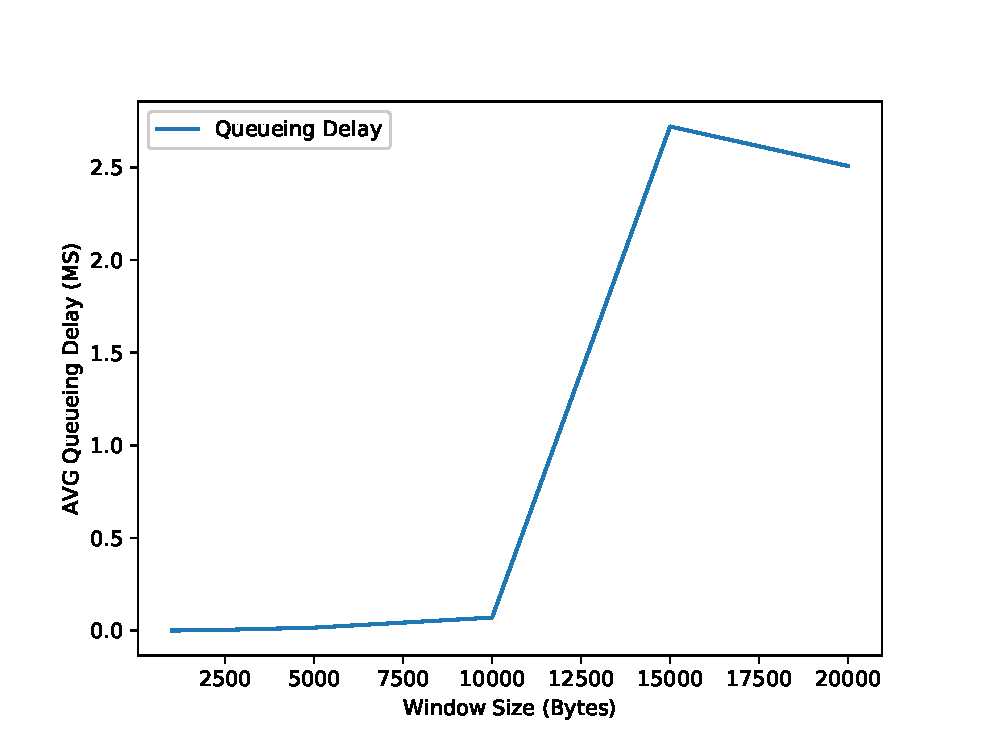
\includegraphics[width=.6\textwidth] {delay.eps}
\end{figure}
%   \caption{Queuing Delay}

\begin{figure}
    \centering
  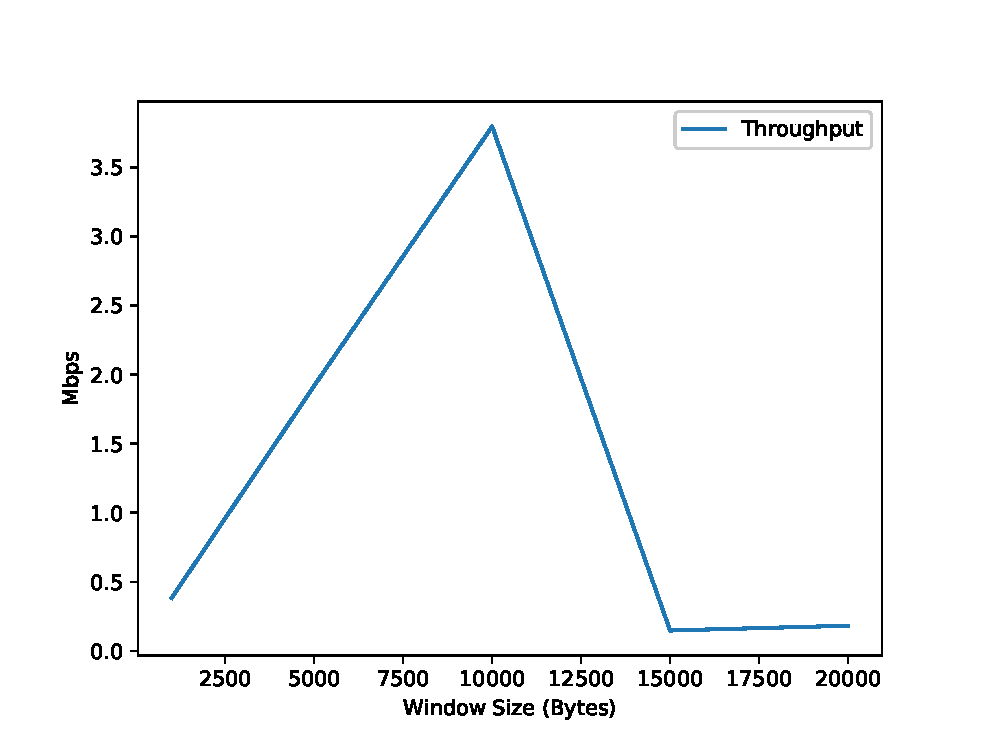
\includegraphics[width=.6\textwidth]{throughput.eps}
\end{figure}
\section{Conclusion}

The experiments showed some interesting results.
The first thing being that dropping packets drastically increases the amount of time needed to send a file over the network but with fast retransmit this time is severely cut.
Another interesting issue is the relationship between the window size and how big the queue is.
It seems the maximum efficiency for out given network is to have the window size be equal to the size of queue on the receiving side.
When you think about this it makes sense the queue on the receiver side will have rarely receive more bytes than the queue can hold. 

\end{document}
